 \section{Metric spaces. Normed vector spaces}

\subsection*{Metric space}
\begin{definition}{Metric $\rho(x,y)$}{}
    Let $X$ be a set. A metric $\rho$ is a function\footnote{metric $\rho$ could be also denoted by $d$. In that way we can call it by `distance'} $\rho: \ X \times X \to [0, \infty)$ such that 
    \begin{enumerate*}
        \item Symmetric
        \[
            \rho(x,y) = \rho(y,x).  
        \]
        \item Positive definite
        \begin{eqnarray}
            &&\rho(x,y) > 0, \ \  x \neq y,\nonumber\\
            &&\rho(x,x) = 0.\nonumber
        \end{eqnarray}
        \item Triangle Inequality
        \[
            \rho(x, z) \leq \rho (x,y) + \rho(y,z).  
        \]
    \end{enumerate*}
\end{definition}

\begin{definition}{Metric space}{}
    A metric space is a set $X$ on which a metric $\rho$ is defined.
\end{definition}

\Ex For $X=\mathbb{R}^n$, $\mathbb{C}^n$, we could define following Euclidean metric

$$
    \rho_E(\vec{x},\vec{y}):=\sqrt{(y_1-x_1)^2+\cdots+(y_n-x_n)^2},
$$
where 
$$
    \vec{x}=
    \begin{bmatrix}
        x_1\\
        \vdots\\
        x_n
    \end{bmatrix},\quad
    \vec{y}=
    \begin{bmatrix}
        y_1\\
        \vdots\\
        y_n
    \end{bmatrix}.
$$

Note that Euclidean metric could be expressed using dot (inner) product as follows 
$$
    \rho_E(\vec{x},\vec{y})=\sqrt{(\vec{x}-\vec{y},\vec{x}-\vec{y})}.
$$

\Ex For $X = \R$, we could define following Euclidean metric
    \[
        \rho(x,y) = \left| e^x - e^y \right|.  
    \]
    
\Ex For $X=\mathbb{R}^n$, we could define following angle metric 
$$
    \rho(\vec{x},\vec{y})=\ \widehat{x,y}\in[0,\pi].
$$

\Ex For discrete set $X$, we could define following discrete metric  
$$
    \rho(x,y)=
    \begin{cases}
        1,\quad x\neq y\\
        0,\quad x=y
    \end{cases}.
$$

\Ex For $X=\mathbb{R}_+:=(0,+\infty)$, we could define following metric 
$$
    \rho(x,y)=|\ln(x)-\ln(y)|.
$$

\Ex For $X=\mathbb{R}^n\setminus \{\vec{0}\}$, we could define following cosine similarity metric 
$$
    \rho(\vec{x},\vec{y})=\cos{(\vec{x},\vec{y})}=\dfrac{(\vec{x},\vec{y})}{\|\vec{x}\| \ \|\vec{y}\|}.
$$
\Ex
    \par 
    For $X = \mathcal{C}[0,1] := \left\{\text{continuous functions } f: [0,1] \to \R\right\}$, we could define following metrics
    \[
            \begin{array}{c}
                \displaystyle\rho_0 (f,g) = \max\limits_{x \in [0,1]} |f(x) - g(x)|,\\
                \displaystyle\rho_1 (f,g) = \int\limits_{0}^1 |f(x) - g(x)|dx,\\
            \rho(f,g) = \rho_0(f,g) + |f(1) - g(1)|.
            \end{array}
    \]
    \begin{figure}[H]
        \centering

% Pattern Info
 


% Pattern Info
 
\tikzset{
pattern size/.store in=\mcSize, 
pattern size = 5pt,
pattern thickness/.store in=\mcThickness, 
pattern thickness = 0.3pt,
pattern radius/.store in=\mcRadius, 
pattern radius = 1pt}
\makeatletter
\pgfutil@ifundefined{pgf@pattern@name@_hx3fdizyv}{
\pgfdeclarepatternformonly[\mcThickness,\mcSize]{_hx3fdizyv}
{\pgfqpoint{0pt}{0pt}}
{\pgfpoint{\mcSize+\mcThickness}{\mcSize+\mcThickness}}
{\pgfpoint{\mcSize}{\mcSize}}
{
\pgfsetcolor{\tikz@pattern@color}
\pgfsetlinewidth{\mcThickness}
\pgfpathmoveto{\pgfqpoint{0pt}{0pt}}
\pgfpathlineto{\pgfpoint{\mcSize+\mcThickness}{\mcSize+\mcThickness}}
\pgfusepath{stroke}
}}
\makeatother

% Pattern Info
 
\tikzset{
pattern size/.store in=\mcSize, 
pattern size = 5pt,
pattern thickness/.store in=\mcThickness, 
pattern thickness = 0.3pt,
pattern radius/.store in=\mcRadius, 
pattern radius = 1pt}
\makeatletter
\pgfutil@ifundefined{pgf@pattern@name@_bfz0rqejm}{
\pgfdeclarepatternformonly[\mcThickness,\mcSize]{_bfz0rqejm}
{\pgfqpoint{0pt}{0pt}}
{\pgfpoint{\mcSize+\mcThickness}{\mcSize+\mcThickness}}
{\pgfpoint{\mcSize}{\mcSize}}
{
\pgfsetcolor{\tikz@pattern@color}
\pgfsetlinewidth{\mcThickness}
\pgfpathmoveto{\pgfqpoint{0pt}{0pt}}
\pgfpathlineto{\pgfpoint{\mcSize+\mcThickness}{\mcSize+\mcThickness}}
\pgfusepath{stroke}
}}
\makeatother

% Pattern Info
 
\tikzset{
pattern size/.store in=\mcSize, 
pattern size = 5pt,
pattern thickness/.store in=\mcThickness, 
pattern thickness = 0.3pt,
pattern radius/.store in=\mcRadius, 
pattern radius = 1pt}
\makeatletter
\pgfutil@ifundefined{pgf@pattern@name@_jnmcvnkyk}{
\pgfdeclarepatternformonly[\mcThickness,\mcSize]{_jnmcvnkyk}
{\pgfqpoint{0pt}{0pt}}
{\pgfpoint{\mcSize+\mcThickness}{\mcSize+\mcThickness}}
{\pgfpoint{\mcSize}{\mcSize}}
{
\pgfsetcolor{\tikz@pattern@color}
\pgfsetlinewidth{\mcThickness}
\pgfpathmoveto{\pgfqpoint{0pt}{0pt}}
\pgfpathlineto{\pgfpoint{\mcSize+\mcThickness}{\mcSize+\mcThickness}}
\pgfusepath{stroke}
}}
\makeatother
\tikzset{every picture/.style={line width=0.75pt}} %set default line width to 0.75pt        

\begin{tikzpicture}[x=0.75pt,y=0.75pt,yscale=-1,xscale=1]
%uncomment if require: \path (0,232); %set diagram left start at 0, and has height of 232

%Straight Lines [id:da8227711206399662] 
\draw [line width=1.5]    (243.97,-31.35) -- (243.97,134.76) ;
\draw [shift={(243.97,-35.35)}, rotate = 90] [fill={rgb, 255:red, 0; green, 0; blue, 0 }  ][line width=0.08]  [draw opacity=0] (6.97,-3.35) -- (0,0) -- (6.97,3.35) -- cycle    ;
%Straight Lines [id:da5452884985398383] 
\draw [line width=1.5]    (599.34,92.5) -- (110.62,92.5) ;
\draw [shift={(603.34,92.5)}, rotate = 180] [fill={rgb, 255:red, 0; green, 0; blue, 0 }  ][line width=0.08]  [draw opacity=0] (6.97,-3.35) -- (0,0) -- (6.97,3.35) -- cycle    ;
%Curve Lines [id:da015320939399488198] 
\draw [line width=1.5]    (145.04,31.03) .. controls (295.79,-94.35) and (356.67,85.44) .. (406.63,110.16) .. controls (456.58,134.88) and (532.02,93.11) .. (569.71,62.12) ;
%Curve Lines [id:da5522362017855642] 
\draw [line width=1.5]    (121.28,106.31) .. controls (187.24,20.78) and (350.64,-48.49) .. (411.51,-16.27) .. controls (472.39,15.96) and (466.99,185.55) .. (584.4,111.59) ;
%Straight Lines [id:da28881118044324894] 
\draw [line width=1.5]  [dash pattern={on 2.25pt off 2.25pt on 2.25pt off 2.25pt}]  (525.28,92.25) -- (526.85,129.13) ;
%Shape: Polygon Curved [id:ds5744246653007492] 
\draw  [draw opacity=0][pattern=_hx3fdizyv,pattern size=6pt,pattern thickness=0.75pt,pattern radius=0pt, pattern color={rgb, 255:red, 0; green, 0; blue, 100}] (492.06,107.4) .. controls (501.38,105.59) and (527.5,94.62) .. (525.28,92.25) .. controls (523.05,89.87) and (527.23,125.01) .. (526.85,129.13) .. controls (526.47,133.25) and (482.74,109.21) .. (492.06,107.4) -- cycle ;
%Shape: Polygon Curved [id:ds08735558984059755] 
\draw  [draw opacity=0][pattern=_bfz0rqejm,pattern size=6pt,pattern thickness=0.75pt,pattern radius=0pt, pattern color={rgb, 255:red, 0; green, 0; blue, 100}] (284.35,-5.14) .. controls (280.85,-10.81) and (397.6,-32.75) .. (407.17,-19.23) .. controls (443.69,-4.86) and (475.72,111.12) .. (485.78,107.03) .. controls (493.9,105.29) and (430.96,127.71) .. (402.44,107.99) .. controls (393.61,101.12) and (311.29,0.96) .. (284.35,-5.14) -- cycle ;
%Shape: Polygon Curved [id:ds5938922303476035] 
\draw  [draw opacity=0][pattern=_jnmcvnkyk,pattern size=6pt,pattern thickness=0.75pt,pattern radius=0pt, pattern color={rgb, 255:red, 0; green, 0; blue, 100}] (247.18,-12.71) .. controls (256.64,-10.11) and (286.37,-4.27) .. (284.35,-5.14) .. controls (282.33,-6.01) and (249.39,6.5) .. (247.18,11.24) .. controls (244.97,15.98) and (237.72,-15.3) .. (247.18,-12.71) -- cycle ;
%Straight Lines [id:da22763832848337806] 
\draw [line width=1.5]  [dash pattern={on 2.25pt off 2.25pt on 2.25pt off 2.25pt}]  (385.3,-23.88) -- (385.3,93.03) ;
%Curve Lines [id:da7796706610264268] 
\draw [line width=1.5]    (442.23,-22.15) .. controls (426.6,-12.18) and (412.83,-10.56) .. (390.46,-5.39) ;
\draw [shift={(386.86,-4.54)}, rotate = 346.53] [fill={rgb, 255:red, 0; green, 0; blue, 0 }  ][line width=0.08]  [draw opacity=0] (6.97,-3.35) -- (0,0) -- (6.97,3.35) -- cycle    ;
%Straight Lines [id:da7973957672218464] 
\draw [line width=1.5]    (310.62,125.43) -- (254.47,1.68) ;
\draw [shift={(252.81,-1.96)}, rotate = 65.59] [fill={rgb, 255:red, 0; green, 0; blue, 0 }  ][line width=0.08]  [draw opacity=0] (6.97,-3.35) -- (0,0) -- (6.97,3.35) -- cycle    ;
%Straight Lines [id:da2771671217924083] 
\draw [line width=1.5]    (310.62,125.43) -- (404.7,82.32) ;
\draw [shift={(408.34,80.65)}, rotate = 155.38] [fill={rgb, 255:red, 0; green, 0; blue, 0 }  ][line width=0.08]  [draw opacity=0] (6.97,-3.35) -- (0,0) -- (6.97,3.35) -- cycle    ;
%Straight Lines [id:da8205617573459223] 
\draw [line width=1.5]    (351.01,133.49) -- (507.98,116.52) ;
\draw [shift={(511.95,116.1)}, rotate = 173.83] [fill={rgb, 255:red, 0; green, 0; blue, 0 }  ][line width=0.08]  [draw opacity=0] (6.97,-3.35) -- (0,0) -- (6.97,3.35) -- cycle    ;

% Text Node
\draw (229.39,97.79) node [anchor=north west][inner sep=0.75pt]   [align=left] {$\displaystyle 0$};
% Text Node
\draw (256.47,-35.05) node [anchor=north west][inner sep=0.75pt]   [align=left] {$\displaystyle y$};
% Text Node
\draw (588.4,71.63) node [anchor=north west][inner sep=0.75pt]   [align=left] {$\displaystyle x$};
% Text Node
\draw (420.27,-38.25) node [anchor=north west][inner sep=0.75pt]   [align=left] {$\displaystyle \rho _{0}( f,g)$};
% Text Node
\draw (294.96,127.01) node [anchor=north west][inner sep=0.75pt]   [align=left] {$\displaystyle \rho _{1}( f,g)$};
% Text Node
\draw (575.28,43.8) node [anchor=north west][inner sep=0.75pt]   [align=left] {$\displaystyle f$};
% Text Node
\draw (591.27,100.23) node [anchor=north west][inner sep=0.75pt]   [align=left] {$\displaystyle g$};
\end{tikzpicture}
\caption*{Figure 1: Geometric interpretation of metrics $\rho_0$ and $\rho_1$}
    \end{figure}
    
\Ex 
Let as consider weighted\footnote{a weighted graph is a graph in which a number (the weight) is assigned to each edge. Such weights might represent for example costs, lengths or capacities, depending on the problem at hand. In our course we consider graphs only with non negatives weights} multigraph\footnote{a multigraph is a graph which is permitted to have multiple edges (also called parallel edges), that is, edges that have the same end nodes} on finite set of nodes $X=\{A,B,C,D, E,F,G,H\}$ (see Figure 2). 
\begin{figure}[h]
    \centering
    \includegraphics[width=0.4\columnwidth]{./lectures/images/multigraph.jpg}
    \caption*{Figure~2:~Weighted multigraph on $X$}
\end{figure}
Let us define metric $\rho(x,y):=$'length of shortest path between points $x$ and $y$'. Then, we have
\begin{eqnarray}
    \rho(A,B)&=&2,\nonumber\\
    \rho(A,A)&=&0,\nonumber\\
    \rho(B,F)&=&4+3+3=10.\nonumber
\end{eqnarray}

~\\ ~\\ ~\\ 
\begin{definition}{Open ball $\overline{B}_R(x_0)$}{}
    An open ball of a radius $R \leq 0$ centered at a pont $c \in X$ is the set
    \[
        \overline{B}_R(c) = \left\{x \in X\ | \ \rho(x,c) < R\right\}.
    \]
\end{definition}

\begin{definition}{Closed ball ${B}_R(x_0)$}{}
    A closed ball of a radius $R\leq 0$ centered at a point $c \in X$ is the set
    \[
        \overline{B}_R(c) = \left\{x \in X \ | \ f(x, c) \leq R\right\}.  
    \]
\end{definition}

\Ex For the graph from the previous example (see Figure 2), we have
\begin{eqnarray}
    \overline{B}_{10}(A)&=&\{A,B,C,D,E\},\nonumber\\
    \overline{B}_{9}(B)&=&\{A,B,C,D,E\},\nonumber\\
    \overline{B}_{10}(B)&=&\{A,B,C,D,E,F\}.\nonumber
\end{eqnarray}

\begin{definition}{Continuous function $f$}{}
    A function $f(x)$ is continuous at a point $x_0$ iff
    \[
        \lim\limits_{x\to x_0} f(x) = y_0.
    \]
    That is $\forall \varepsilon > 0 \ \exists \delta>0$
    \[
        f\left(B_{\delta}(x_0)\right) \subset B_\varepsilon\left(f(x_0)\right).
    \]
\end{definition}

\Ex For $X=\mathbb{R}$, we could define non continuous metric
    \[
        \rho(x,y) = \left\{
            \begin{array}{cl}
                1, & x-y \in \Q \\
                2, & x -y \notin \Q\\
                0, & x = y
            \end{array}.
        \right. 
    \]
    We see that function $\rho$ is not continuous at any point. At the same time, function $\rho$ is metric, since $\rho$ is 
    \begin{enumerate*}
        \item Symmetric, because
        \begin{eqnarray}
            x-y\in Q \Leftrightarrow y-x\in Q,\nonumber\\
            x-y\notin Q \Leftrightarrow y-x\notin Q.\nonumber
        \end{eqnarray}
        \item Positive definite, because
        \begin{eqnarray}
            &&\rho(x,y) > 0, \ \  x \neq y,\nonumber\\
            &&\rho(x,x) = 0.\nonumber
        \end{eqnarray}
        \item Triangle Inequality, because 
        \begin{enumerate}
            \item If $x\notin Q$ (similarly for $z\notin Q$) and $z\neq x$, then 
            \begin{eqnarray}
                &\rho(x,z)\leq \rho(x,y)+ \rho(y,z)&\nonumber\\
                &\Leftrightarrow&\nonumber\\
                &2 \leq 2 + \rho (y,z),&\nonumber
            \end{eqnarray}
            which holds for any $x$ and $y$.
            \item  If $x,z\in Q$ and $x\neq z$
            \begin{eqnarray}
                &\rho(x,z)\leq \rho(x,y)+ \rho(y,z)&\nonumber\\
                &\Leftrightarrow&\nonumber\\
                &1 \leq \rho (x,y) + \rho (x,y),&\nonumber
        \end{eqnarray}
            which holds for $y$.
        \end{enumerate}
    \end{enumerate*}

\newpage
\subsection*{Normed vector space}
\begin{definition}{Norm}{}
    Let $V$ be a vector space. A norm $\nu$ is a function\footnote{for $v\in V$ norm also could be denoted by $\|v\|:=\nu(v)$} $\nu: \ V \to \R$, such that 
    \begin{enumerate*}
        \item Positive definite
        \[ 
            \nu\left(\vec{x}\right) > 0,\quad x\neq\vec{0}.
        \]
        \item Homogeneity \[
            \nu\left(\alpha \vec{x}\right) = |\alpha|\nu\left(\vec{x}\right).
        \]
        \item Triangle inequality
        \[ 
            \nu\left(\vec{x} + \vec{y}\right) \leq \nu\left(\vec{x}\right) + \nu\left(\vec{y}\right).
        \]
    \end{enumerate*}
\end{definition}
\begin{definition}{Normed vector space}{}
    A normed vector space is a vector space $V$ on which a norm $\nu$ is defined.
\end{definition}


\begin{definition}{ Euclidean norm  $\|\vec{x}\|_2$}{}
    For $V=\mathbb{R}^n,\mathbb{C}^n$, we could define Euclidean norm
        \[
            \left|\vec{x}\right|_2 :=\rho_E(\vec{0},\vec{x})= \sqrt{\sum\limits_{i=1}^n |x_i|^2}.    
        \]
\end{definition}

\begin{lemma}{}{}
    Let $\nu$ be a norm, then 
    $\nu\left(\vec{0}\right) = 0$.
\end{lemma}
\begin{proof}
    $\nu\left(\vec{0}\right)=\nu\left(0 \cdot \vec{0}\right) = 0 \cdot \nu\left(\vec{0}\right) = 0.$
\end{proof}
    
\begin{proposition}{}{}
    Let a normed vector space and it's norm be $V$ and $\nu$ respectively. Then a function $\rho\left(\vec{x},\vec{y}\right) := \nu\left(\vec{y} - \vec{x}\right)$ is a metric. 
\end{proposition}
\begin{proof}
    \begin{enumerate}
        \item Positive definition
        \begin{eqnarray}
                \displaystyle\rho\left(\vec{x}, \vec{y}\right) &=& \nu\left(\vec{y} - \vec{x}\right) > 0, \nonumber\\
                \displaystyle \rho\left(\vec{x}, \vec{x}\right) &=& \nu\left(\vec{x} - \vec{x}\right) = \nu\left(\vec{0}\right) \stackrel{\text{Lemma}}{=} 0.\nonumber
        \end{eqnarray}
        \item Symmetric
        \begin{eqnarray}
            \rho\left(\vec{x}, \vec{y}\right) 
            &=& \nu\left(\vec{y} - \vec{x}\right) \nonumber\\
            &=& |-1|\nu\left(\vec{x} - \vec{y}\right) \nonumber\\
            &=& \nu\left(\vec{x} - \vec{y}\right) \nonumber\\
            &=& \rho\left(\vec{y}, \vec{x}\right) \nonumber.
        \end{eqnarray}
        \item Triangle inequality
        \begin{eqnarray}
                \rho\left(\vec{x}, \vec{y}\right) + \rho\left(\vec{y}, \vec{z}\right) 
                &=&  
                \nu\left(\vec{y} - \vec{x}\right) + \nu\left(\vec{z} - \vec{y}\right)  \nonumber\\
                &\geq&  \nonumber
                \nu\left(\vec{y} - \vec{x} + \vec{z} -\vec{y} \right) \nonumber\\
                &=&  \nu\left(\vec{z} - \vec{x}\right) \nonumber\\
                &=&  \rho\left(\vec{x}, \vec{z}\right) \nonumber.
        \end{eqnarray}
    \end{enumerate}
\end{proof}
\begin{note}{}{}
    Any normed space is a metric space.
\end{note}

\begin{definition}{Manhattan norm (or Taxicab norm) $\|\vec{x}\|_1$}{}
        For  vector space $V=\R^n, \C^n$, we could define Manhattan norm (or Taxicab norm)
        $$
            \|\vec{x}\|_1 := \sum\limits_{i=1}^n |x_i|.  
        $$
    \end{definition}
\begin{proof}
    {
    \begin{wrapfigure}{r}{0.3\textwidth}
        \scalebox{0.8}{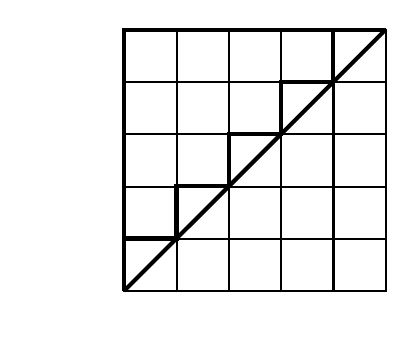
\begin{tikzpicture}[x=0.75pt,y=0.75pt,yscale=-1,xscale=1]
            \path (0,164); %set diagram left start at 0, and has height of 164
            
            %Shape: Grid [id:dp08042200947302103] 
            \draw  [draw opacity=0][line width=0.75]  (46.53,16.6) -- (172.55,16.6) -- (172.55,142.61) -- (46.53,142.61) -- cycle ; \draw  [line width=0.75]  (71.74,16.6) -- (71.74,142.61)(96.94,16.6) -- (96.94,142.61)(122.14,16.6) -- (122.14,142.61)(147.34,16.6) -- (147.34,142.61) ; \draw  [line width=0.75]  (46.53,41.8) -- (172.55,41.8)(46.53,67.01) -- (172.55,67.01)(46.53,92.21) -- (172.55,92.21)(46.53,117.41) -- (172.55,117.41) ; \draw  [line width=0.75]  (46.53,16.6) -- (172.55,16.6) -- (172.55,142.61) -- (46.53,142.61) -- cycle ;
            %Straight Lines [id:da6909809940649061] 
            \draw [line width=1.5]    (46.53,142.34) -- (172.43,16.6) ;
            %Straight Lines [id:da10608550876089407] 
            \draw [line width=1.5]    (46.53,142.34) -- (46.53,117.19) -- (71.71,117.19) -- (71.71,92.04) -- (96.89,92.04) -- (96.89,66.89) -- (122.07,66.89) -- (122.07,41.75) -- (147.25,41.75) -- (147.25,16.6) -- (172.43,16.6) ;
            %Straight Lines [id:da694529903122499] 
            \draw [line width=1.5]    (172.43,16.6) -- (46.53,16.6) -- (46.53,142.34) ;
            \end{tikzpicture}}
            \caption*{Figure~3:~Geometric~interpretation of~Manhattan~norm~$\|\vec{x}\|_1$}
    \end{wrapfigure}
    Let's prove that function $\|x\|_1$ is a norm.
    \begin{enumerate}
        \item Positive definite property:
        Let $x \in \R^n$ or $x \in \C^n$. Obviously $||x||_1 \geq 0.$ Also $||x||_1 = 0$ iff $x = 0$.
        \item Homogeneity property
        \useshortskip
        \[
            \forall c \in \R: \ ||c\cdot x||_1 = \sum\limits_{i=1}^n |c\cdot x_i| = |c| \cdot \sum\limits_{i=1}^n |x_i| = |c| \cdot ||x||_1 .
        \]
    \end{enumerate}}

    ~\\
    \begin{enumerate}
        \item[3.] Triangle inequality $\forall x, y \in \R^n$:
        \[
            \begin{array}{c}
                \displaystyle ||x+y||_1 = \sum\limits_{i=1}^n |x_i + y_i| \leq \sum\limits_{i=1}^n \left(|x_i| + |y_i|\right) =               \sum\limits_{i=1}^n |x_i| + \sum\limits_{i=1}^n |y_i| = ||x||_1 + ||y||_1.     
            \end{array}
        \]
    \end{enumerate}
\end{proof}

 \begin{definition}{Maximum norm (or Infinity norm) $\|\vec{x}\|_\infty$}{}
    For  vector space $V=\R^n, \C^n$, we could define Maximum norm (or Infinity norm)~ ~  ~  ~  ~  ~  ~  ~  ~  ~  ~ 
            \[
                \|\vec{x}\|_\infty = \max\limits_{1 \leq i \leq n} |x_i|.  
            \]
    \end{definition}
\begin{proof}
        Let's prove that function $\|\vec{x}\|_\infty$ is a norm.
        \begin{enumerate}
            \item The function $||x||_\infty$ is positive since it is the maximum over a set of positive terms $|x_i|$.
            \item Homogeneity property
            \[
                ||\alpha\cdot x ||_{\infty} = \max\limits_{1 \leq i \leq n} |\alpha\cdot x_i| = \max\limits_{1 \leq i \leq n} |\alpha| \cdot |x_i| = |\alpha| \cdot \max\limits_{1 \leq i \leq n} = |\alpha|\cdot ||x||_\infty. 
            \]
            \item Triangle inequality
            \[
                ||x+y||_{\infty} = \max\limits_{1 \leq i \leq n} |x_i + y_i| \leq \max\limits_{1 \leq i \leq n} \left(|x_i| + |y_i|\right) \leq \max\limits_{1 \leq i \leq n} |x_i| + \max\limits_{1 \leq i \leq n} |y_i| = ||x||_\infty + ||y||_\infty.
            \]
        \end{enumerate}
\end{proof}

\begin{definition}{Minkovskiy $p-$norm $\|\vec{x}\|_p$}{}
For vector space of continuous functions $V=\R^n, \C^n$, we could define Minkovskiy $p-$norm
\[
    \|\vec{x}\|_p = \sqrt[P]{\sum\limits_{i=1}^n |x_i|^p}, \quad p\geq 1.
\]
\end{definition}
\begin{wrapfigure}{r}{0.4\columnwidth}
    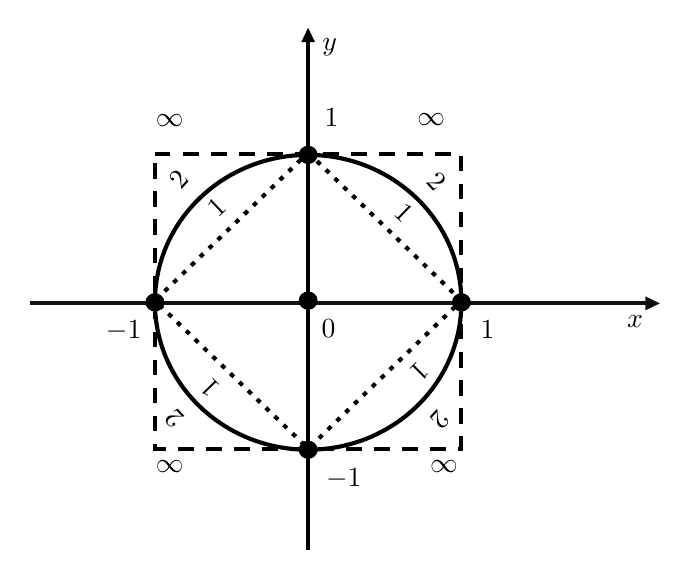
\begin{tikzpicture}[x=0.75pt,y=0.75pt,xscale=1, yscale=-1]
        %uncomment if require: \path (0,300); %set diagram left start at 0, and has height of 300
        
        %Straight Lines [id:da8306888936977477] 
        \draw [line width=1.5]    (175.02,17) -- (175.02,264.39) ;
        \draw [shift={(175.02,13)}, rotate = 90] [fill={rgb, 255:red, 0; green, 0; blue, 0 }  ][line width=0.08]  [draw opacity=0] (6.97,-3.35) -- (0,0) -- (6.97,3.35) -- cycle    ;
        %Straight Lines [id:da5110121506356493] 
        \draw [color={rgb, 255:red, 16; green, 16; blue, 16 }  ,draw opacity=1 ][fill={rgb, 255:red, 4; green, 4; blue, 4 }  ,fill opacity=1 ][line width=1.5]    (340.5,145.77) -- (40.89,145.77) ;
        \draw [shift={(344.5,145.77)}, rotate = 180] [fill={rgb, 255:red, 16; green, 16; blue, 16 }  ,fill opacity=1 ][line width=0.08]  [draw opacity=0] (6.97,-3.35) -- (0,0) -- (6.97,3.35) -- cycle    ;
        %Shape: Ellipse [id:dp06424647272445538] 
        \draw  [line width=1.5]  (101.19,145.27) .. controls (101.19,106.04) and (134.25,74.24) .. (175.02,74.24) .. controls (215.8,74.24) and (248.85,106.04) .. (248.85,145.27) .. controls (248.85,184.49) and (215.8,216.29) .. (175.02,216.29) .. controls (134.25,216.29) and (101.19,184.49) .. (101.19,145.27) -- cycle ;
        %Shape: Rectangle [id:dp9119970932820067] 
        \draw  [dash pattern={on 5.63pt off 4.5pt}][line width=1.5]  (101.19,73.71) -- (248.85,73.71) -- (248.85,215.76) -- (101.19,215.76) -- cycle ;
        %Shape: Diamond [id:dp4333715282427959] 
        \draw  [dash pattern={on 1.69pt off 2.76pt}][line width=1.5]  (175.02,73.14) -- (248.85,144.45) -- (175.02,215.76) -- (101.19,144.45) -- cycle ;
        %Shape: Ellipse [id:dp8226317539510353] 
        \draw  [fill={rgb, 255:red, 0; green, 0; blue, 0 }  ,fill opacity=1 ] (170.74,144.45) .. controls (170.74,142.18) and (172.66,140.33) .. (175.02,140.33) .. controls (177.39,140.33) and (179.31,142.18) .. (179.31,144.45) .. controls (179.31,146.73) and (177.39,148.58) .. (175.02,148.58) .. controls (172.66,148.58) and (170.74,146.73) .. (170.74,144.45) -- cycle ;
        %Shape: Ellipse [id:dp08502683026718438] 
        \draw  [fill={rgb, 255:red, 0; green, 0; blue, 0 }  ,fill opacity=1 ] (244.57,145.27) .. controls (244.57,142.99) and (246.49,141.14) .. (248.85,141.14) .. controls (251.22,141.14) and (253.14,142.99) .. (253.14,145.27) .. controls (253.14,147.54) and (251.22,149.39) .. (248.85,149.39) .. controls (246.49,149.39) and (244.57,147.54) .. (244.57,145.27) -- cycle ;
        %Shape: Ellipse [id:dp4574361474994544] 
        \draw  [fill={rgb, 255:red, 0; green, 0; blue, 0 }  ,fill opacity=1 ] (96.91,145.27) .. controls (96.91,142.99) and (98.82,141.14) .. (101.19,141.14) .. controls (103.56,141.14) and (105.48,142.99) .. (105.48,145.27) .. controls (105.48,147.54) and (103.56,149.39) .. (101.19,149.39) .. controls (98.82,149.39) and (96.91,147.54) .. (96.91,145.27) -- cycle ;
        %Shape: Ellipse [id:dp9128016551294487] 
        \draw  [fill={rgb, 255:red, 0; green, 0; blue, 0 }  ,fill opacity=1 ] (170.74,74.24) .. controls (170.74,71.96) and (172.66,70.11) .. (175.02,70.11) .. controls (177.39,70.11) and (179.31,71.96) .. (179.31,74.24) .. controls (179.31,76.51) and (177.39,78.36) .. (175.02,78.36) .. controls (172.66,78.36) and (170.74,76.51) .. (170.74,74.24) -- cycle ;
        %Shape: Ellipse [id:dp34957400582859055] 
        \draw  [fill={rgb, 255:red, 0; green, 0; blue, 0 }  ,fill opacity=1 ] (170.74,216.29) .. controls (170.74,214.02) and (172.66,212.17) .. (175.02,212.17) .. controls (177.39,212.17) and (179.31,214.02) .. (179.31,216.29) .. controls (179.31,218.57) and (177.39,220.42) .. (175.02,220.42) .. controls (172.66,220.42) and (170.74,218.57) .. (170.74,216.29) -- cycle ;
        
        % Text Node
        \draw (180.27,152.42) node [anchor=north west][inner sep=0.75pt]   [align=left] {$\displaystyle 0$};
        % Text Node
        \draw (76.36,152.67) node [anchor=north west][inner sep=0.75pt]   [align=left] {$\displaystyle -1$};
        % Text Node
        \draw (256.83,152.67) node [anchor=north west][inner sep=0.75pt]   [align=left] {$\displaystyle 1$};
        % Text Node
        \draw (182.38,223.97) node [anchor=north west][inner sep=0.75pt]   [align=left] {$\displaystyle -1$};
        % Text Node
        \draw (181.75,50.91) node [anchor=north west][inner sep=0.75pt]   [align=left] {$\displaystyle 1$};
        % Text Node
        \draw (226.43,53) node [anchor=north west][inner sep=0.75pt]   [align=left] {$\displaystyle \infty $};
        % Text Node
        \draw (232.5,220.22) node [anchor=north west][inner sep=0.75pt]   [align=left] {$\displaystyle \infty $};
        % Text Node
        \draw (100.43,220.22) node [anchor=north west][inner sep=0.75pt]   [align=left] {$\displaystyle \infty $};
        % Text Node
        \draw (100.43,53.73) node [anchor=north west][inner sep=0.75pt]   [align=left] {$\displaystyle \infty $};
        % Text Node
        \draw (221.69,94.87) node [anchor=north west][inner sep=0.75pt]  [rotate=-43.96] [align=left] {$\displaystyle 1$};
        % Text Node
        \draw (123.83,98.41) node [anchor=north west][inner sep=0.75pt]  [rotate=-316.59] [align=left] {$\displaystyle 1$};
        % Text Node
        \draw (126.89,193.78) node [anchor=north west][inner sep=0.75pt]  [rotate=-225.71] [align=left] {$\displaystyle 1$};
        % Text Node
        \draw (235.69,179.51) node [anchor=north west][inner sep=0.75pt]  [rotate=-135.19] [align=left] {$\displaystyle 1$};
        % Text Node
        \draw (105.42,86.05) node [anchor=north west][inner sep=0.75pt]  [rotate=-311.39] [align=left] {$\displaystyle 2$};
        % Text Node
        \draw (237.7,79.66) node [anchor=north west][inner sep=0.75pt]  [rotate=-47.02] [align=left] {$\displaystyle 2$};
        % Text Node
        \draw (245.64,202.2) node [anchor=north west][inner sep=0.75pt]  [rotate=-133.09] [align=left] {$\displaystyle 2$};
        % Text Node
        \draw (109.66,208.34) node [anchor=north west][inner sep=0.75pt]  [rotate=-226.72] [align=left] {$\displaystyle 2$};
        % Text Node
        \draw (327.49,150.48) node [anchor=north west][inner sep=0.75pt]   [align=left] {$\displaystyle x$};
        % Text Node
        \draw (180.61,16.85) node [anchor=north west][inner sep=0.75pt]   [align=left] {$\displaystyle y$};
        \end{tikzpicture}
        \caption*{Figure 4: Unit balls for norms $\|\cdot\|_1, \|\cdot\|_2$ and $\|\cdot\|_\infty$}
    \end{wrapfigure}   
The notations $||\cdot ||_1, ||\cdot||_2$ and $||\cdot ||_\infty$ are justified because of the fact that all these norms are special cases of the general Minkovskiy $p-$norm.
~\\~\\~\\~\\~\\~\\~\\~\\~\\~\\~\\~\\~\\~\\~\\~\\~\\~\\
\Ex For the vector $\vec{x} = \begin{bmatrix}
    1 \\
    2 \\ 
    -3 \\
    5
\end{bmatrix}$, we have
\[
    \|\vec{x}\|_1 = 11, \quad \|\vec{x}\|_2 = \sqrt{39}, \quad 
    \|\vec{x}\|_\infty = 5.
\]

For the vector $\vec{y} = \begin{bmatrix}
    1+i \\
    2-3i\\
    4
\end{bmatrix}$, we have
\[
    \|\vec{y}\|_1 = \sqrt{2} + \sqrt{13} + 4, \quad \|\vec{y}\|_2 = \sqrt{31}, \quad \|\vec{y}\|_\infty = 4.  
\]

\begin{definition}{$p-$norm $\|\vec{x}\|_p$ for $\mathcal{C}[a,b]$}{}
    For vector space $V=\mathcal{C}[a,b]$, we could define norms 
    \begin{eqnarray} 
        ||f||_1 &=& \int\limits_{a}^b |f(x)| dx,\nonumber\\
        ||f||_2 &=& \sqrt{\int\limits_a^b f^2(x)dx},\nonumber\\
        ||f||_\infty &=& \max\limits_{x\in [a,b]} |f(x)|,\nonumber\\
        ||f||_p &=& \sqrt[p]{\int\limits_{a}^b |f(x)|^p dx}. \nonumber
    \end{eqnarray}
\end{definition}

\Ex For $V = \mathcal{C}[0,1]$, we have
\begin{eqnarray}
        \displaystyle ||f||_p &=& \sqrt[p]{\int\limits_{0}^1 |f(x)|^p dx},  \nonumber\\
        \displaystyle ||f||_1 &=& \int\limits_{0}^1 |f(x)| dx,\nonumber\\
        \displaystyle ||f||_\infty &=& \displaystyle ||f||_0 =\max\limits_{x \in [0,1]} |f(x)|.\nonumber
\end{eqnarray}

\begin{definition}{Weighted norms for $ \mathcal{C}[0,1]$}{}
    For vector space $V = \mathcal{C}[0,1]$ and $\omega \geq 0$, we could define weighted norms
    \begin{eqnarray}
        \displaystyle ||f||_p^\omega &=& \sqrt[p]{\int\limits_0^1 |f(x)|^p \cdot \omega(x) dx}, \nonumber\\
        \displaystyle ||f||_\infty^\omega = ||f||_0^\omega &=& \max\limits_{x\in [0,1]} |f(x) \cdot \omega(x)|.\nonumber
    \end{eqnarray}
\end{definition}

\subsection*{Balls in normed space}
Let $V$ be a normed vector space. Let $\rho(x,y):=\nu(x-y)$ be a metric induced by norm $\nu$ on $V$. Then,
$$
    B_{R}(c)
    =
    \{x \ | \ \rho(x,c)\leq R \}
    =
    \{x \ | \ \nu(x-c)\leq R \}
$$
\begin{proposition}{}{}
    Let $V$ be a normed space.
    \begin{enumerate}
        \item Any two balls $B_R(\vec{x})$ and $B_R(\vec{y})$,  are congruent (same geometric figures). That is, there is a parallel translation $\vec{x} \mapsto \vec{x}+\vec{v}$, which maps one ball onto another. Specifically, we mean that 
        $$B_R(\vec{x})+\vec{v}=B_R(\vec{y}).$$
        
        \item For any two balls $B_R(\vec{c})$ and $B_r(\vec{c})$, there is a homothety $\vec{x} \mapsto \lambda \vec{x}$, which transfers one ball onto another. Specifically, we mean that 
        $$B_R(\vec{c}) = \lambda B_r(\vec{c}).$$
    \end{enumerate}
\end{proposition}
\begin{proof}
    \begin{enumerate}
        \item Let $v=\vec{y}-\vec{x}$, then we have
        \begin{eqnarray}
               B_R(\vec{x}) + \vec{v} 
               &=& \left\{\vec{a}\ | \ \nu\left(\vec{a} - \vec{x}\right) \leq R\right\} + \left(\vec{y} - \vec{x}\right)  \nonumber\\ 
               &=& \left\{\vec{a} + \vec{y} - \vec{x}\ | \ \nu\left(\vec{a} - \vec{x}\right) \leq R\right\} \nonumber\\
               &=& \left\{\vec{b}\ | \ \nu\left(\vec{b} - \vec{y}\right) \leq R \right\} \nonumber\\
               &=& B_R(\vec{y}), \nonumber
        \end{eqnarray}
        where $\vec{y}= \vec{b} - \vec{a} - \vec{x}$.
        \item Let $\lambda=\dfrac{R}{r}$, then we have
        \begin{eqnarray}    
                 \lambda  B_r(\vec{c}) &=& \dfrac{R}{r}\cdot \left\{\vec{a}\ | \ \nu\left(\vec{a}-\vec{c}\right) \leq r\right\} \nonumber\\
                  &=& \left\{\dfrac{R}{r} \cdot \vec{a} \ | \ \nu\left(\vec{a}\right) \leq r\right\} \nonumber\\
                 &=& \left\{\vec{b}\ | \ \nu\left(\dfrac{r}{R} \cdot \vec{b}\right) \leq r\right\} \nonumber\\
                 &=& \left\{\vec{b}\ | \ \dfrac{r}{R} \cdot \nu \left(\vec{b}\right) \leq r\right\} \nonumber
        \end{eqnarray}
        \begin{eqnarray}           
                 &=& \left\{\vec{b}\ | \ \nu\left(\vec{b}\right) \leq \dfrac{r\cdot R}{r}\right\} \nonumber\\
                  &=&\left\{\vec{b} \ | \ \nu\left(\vec{b}\right) \leq R\right\}\nonumber \\
                &=& B_R(\vec{c}).\nonumber 
        \end{eqnarray}
    \end{enumerate}
\end{proof}
\begin{definition}{Inner product}{}
    An inner product on a real vector space $V$ is a function
    $$
    (\cdot,\cdot): V\times V\rightarrow \mathbb{R},
    $$
    such that $\forall \vec{x},\vec{y},\vec{z}\in V, \alpha,\beta\in\mathbb{R}$    
    \begin{enumerate*}
        \item Symmetric
        \[ 
            (\vec{x},\vec{y})=(\vec{y},\vec{x}).
        \]
        \item Linear \[
            (\alpha\vec{x}+\beta\vec{y},\vec{z})=
            \alpha(\vec{x},\vec{z})+\beta(\vec{y},\vec{z}).
        \]
        \item Positive-definite
        \[ 
            (\vec{x},\vec{x})>0, \quad \vec{x}\neq \vec{0}.
        \]
    \end{enumerate*}
\end{definition}

\begin{theorema}{Inner product and norm}{}
\begin{enumerate}
    \item If norm $\| \cdot\|$ is Euclidean, then parallelogram rule holds. That is,
    $$
        2\|\vec{a}\|^2+2\|\vec{b}\|^2=\|\vec{a}+\vec{b}\|^2+\|\vec{a}-\vec{b}\|^2.
    $$
    \item If parallelogram rule holds, then a norm $\| \cdot\|$ is Euclidean. That is,
    $$
        (\vec{a},\vec{b})=\dfrac{\|\vec{a}+\vec{b}\|^2-\|\vec{a}\|^2-\|\vec{b}\|^2}{2},
    $$
    defines inner product on vector space $V$.
\end{enumerate}
\end{theorema}
\Ex Let us consider vector space $\mathbb{R}^2$. Let us define following norm $\|\cdot\|$ on $\mathbb{R}^2$ 
$$
    \left\| 
    \begin{matrix}
        x \\
        y
    \end{matrix}
    \right\| = \sqrt{x^2-2xy+5y^2}.
$$
Then corresponding inner product $(\vec{a},\vec{b})$ of arbitrary vectors $\vec{a}=\begin{bmatrix}
    x_1\\
    y_1
\end{bmatrix},\vec{b}=\begin{bmatrix}
    x_2\\
    y_2
\end{bmatrix}\in\mathbb{R}^2$ is the following 
\begin{eqnarray}
    (\vec{a},\vec{b})&=&\dfrac{\|\vec{a}+\vec{b}\|^2-\|\vec{a}\|^2-\|\vec{b}\|^2}{2}\nonumber\\
    &=&
    \dfrac{(x_1+x_2)^2-2(x_1+x_2)(y_1+y_2)+5(y_1+y_2)^2}{2}
    -\dfrac{x_1^2-2x_1y_1+5y_1^2}{2}
    -\dfrac{x_2^2-2x_2y_2+5y_2^2}{2}\nonumber\\
    &=&
    x_1x_2-x_1y_2-x_2y_1+10y_1y_2.\nonumber
\end{eqnarray}
